\documentclass{article}
\usepackage[portuges]{babel}
\usepackage[utf8]{inputenc}
\usepackage[margin=1in, includefoot,footskip=30pt,]{geometry} %Equivalente a fullpage sem estragar o cabeçalho e rodapé

\usepackage{graphicx} %Permite inserir imagens
\usepackage{mathtools} % mathtools loads the amsmath package automatically
\usepackage{amssymb}

\DeclarePairedDelimiter\abs{\lvert}{\rvert}%
\DeclarePairedDelimiter\norm{\lVert}{\rVert}%

\usepackage{float}

\usepackage[hidelinks=true]{hyperref}

\usepackage{enumitem} % Permite adicionar tab a itemizes
\usepackage{indentfirst}
\usepackage{subcaption}


% ----- Definiçoes para as tabelas -----
\usepackage{tabularx}
\newcolumntype{Y}{>{\centering\arraybackslash}X}


% ----- Cabeçalho e rodapé -----
\usepackage{color}
%\usepackage{xcolor}
\definecolor{light-gray}{gray}{0.80}
\definecolor{mylight-gray}{gray}{0.30}

\usepackage{fancyhdr}
\pagestyle{fancy}
\fancyhf{}

\renewcommand{\headrulewidth}{1pt}
\renewcommand{\footrulewidth}{0.5pt}

\rhead{\textbf{\large{\textbf{\textsc{Algoritmia e Desempenho em Redes de Computadores}}}} \\ \textsc{Inter-domain routing}}
\lhead{
\includegraphics[scale=0.7]{capa/IST_Logo.png}}
\rfoot{\textsc{\textcolor{mylight-gray}{Página} \thepage}}

\usepackage{etoolbox}
\patchcmd{\headrule}{\hrule}{\color{light-gray}\hrule}{}{}
\patchcmd{\footrule}{\hrule}{\color{light-gray}\hrule}{}{}


% ----- Comandos Personalizados -----
\newcommand{\betamaisum}[0]{\ensuremath{\left( \beta + 1 \right)}}

\newcommand{\volt}[0]{\ensuremath{\ V}}
\newcommand{\mvolt}[0]{\ensuremath{\ mV}}
\newcommand{\uvolt}[0]{\ensuremath{\ \mu V}}

\newcommand{\amp}[0]{\ensuremath{\ A}}
\newcommand{\mamp}[0]{\ensuremath{\ mA}}
\newcommand{\uamp}[0]{\ensuremath{\ \mu A}}

\newcommand{\mohm}[0]{\ensuremath{\ m \Omega}}
\newcommand{\ohm}[0]{\ensuremath{\ \Omega}}
\newcommand{\kohm}[0]{\ensuremath{\ k\Omega}}

\newcommand{\siemen}{\ensuremath{\ S}}
\newcommand{\msiemen}{\ensuremath{\ mS}}
\newcommand{\usiemen}{\ensuremath{\ \mu S}}
\newcommand{\Msiemen}{\ensuremath{\ MS}}

\newcommand{\pfarad}{\ensuremath{\ pF}}
\newcommand{\ufarad}{\ensuremath{\ \mu F}}
\newcommand{\nfarad}{\ensuremath{\ nF}}

\newcommand{\Hz}{\ensuremath{\ Hz}}
\newcommand{\kHz}{\ensuremath{\ kHz}}

\newcommand{\dB}{\ensuremath{\ dB}}


\newcommand{\dez}[1]{\ensuremath{\cdot 10^{#1}}}

\newcommand{\barravertical}{\ensuremath{\biggr\rvert}}

% ----- Template para secções subsecções -----
\usepackage[explicit]{titlesec}
\usepackage{color, colortbl}
\usepackage[usenames,dvipsnames]{xcolor}

\titleformat{\section}
	{\normalfont\Large\scshape}{}{0em}{%\setlength
	%\fboxsep{9pt}
	%\colorbox{NavyBlue}
	{\parbox{\dimexpr\textwidth-2\fboxsep\relax}{
	\ifnum\thesection>0
		\thesection\quad#1
	\else
		#1
	\fi}}}

\titleformat{\subsection}{\normalfont\scshape\large}{}{0em}{{#1}}%\thesubsection \ #1}}
\titleformat{\subsubsection}{\normalfont\scshape}{}{0em}{{#1}}%\thesubsubsection \ #1}}
\titleformat{\paragraph}{\normalfont\scshape\small}{}{0em}{{#1}}

%\newcommand{\sectionbreak}{\clearpage} %Faz page break antes de cada secção

\usepackage{pdfpages}

\usepackage{xcolor}
\usepackage{pgfplots}
\usepackage{tikz}

% Define bar chart colors
%
\definecolor{bblue}{HTML}{4F81BD}
\definecolor{rred}{HTML}{C0504D}
\definecolor{ggreen}{HTML}{9BBB59}
\definecolor{ppurple}{HTML}{9F4C7C}



\usepackage{algpseudocode}
\usepackage{algorithm}

\makeatletter
\renewcommand{\ALG@name}{Algoritmo}
\makeatother

\makeatletter
\newenvironment{breakablealgorithm}
  {% \begin{breakablealgorithm}
   \begin{center}
     \refstepcounter{algorithm}% New algorithm
     \hrule height.8pt depth0pt \kern2pt% \@fs@pre for \@fs@ruled
     \renewcommand{\caption}[2][\relax]{% Make a new \caption
       {\raggedright\textbf{\ALG@name~\thealgorithm} ##2\par}%
       \ifx\relax##1\relax % #1 is \relax
         \addcontentsline{loa}{algorithm}{\protect\numberline{\thealgorithm}##2}%
       \else % #1 is not \relax
         \addcontentsline{loa}{algorithm}{\protect\numberline{\thealgorithm}##1}%
       \fi
       \kern2pt\hrule\kern2pt
     }
  }{% \end{breakablealgorithm}
     \kern2pt\hrule\relax% \@fs@post for \@fs@ruled
   \end{center}
  }
\makeatother


% ----- DOCUMENTO -----
\begin{document}

% Inclui a capa (existem pacotes especificos que interferem com os existentes neste documento)

\includepdf[pages={1}]{capa/capa.pdf}
\setcounter{page}{1}

\subsection{Algoritmo \texttt{CommercialRoute}}

Com este algoritmo pretende-se descobrir qual o tipo de rota comercial mais favorável a um determinado domínio para chegar a um dado domínio de destino.

\begin{algorithm}[H]
\caption{}
\label{al:generatecode}
\begin{algorithmic}
\Function{CommercialRoute}{$s$, $isTopologyConnected$}
	\For {all vertices $v$}
		\State $visisted[v] := false$
		\State $route\_vector[v] :=$ \textbf{if} $isTopologyConnected$ \textbf{then} $Provider$ \textbf{else} $None$

	\EndFor
	
	\State $domain := s$; $route\_vector[s] := Itself$
	
	\State $fifo\_clients := \emptyset$; 
	$fifo\_peers := \emptyset$;
	$fifo\_providers := \emptyset$
	
	\State
	
	\While{$domain \neq NIL $}
		\State $visisted[domain] := true$
		
		\If { \textbf{not} $isTopologyConnected$}
			\State $fifo\_providers := fifo\_providers \ \cup$ all vertices $v$ clients of $domain$
		\EndIf
						
		\If {$route\_vector[domain] = Client$ \textbf{or} $route\_vector[domain] = Itself$}
			\State $fifo\_peers := fifo\_peers \ \cup$ all vertices $v$ peers of $domain$			
			\State $fifo\_clients := fifo\_clients \ \cup$ all vertices $v$ providers of $domain$		
		\EndIf
		
		
		\State $domain :=$ Remove a vertice $v$ from $fifo\_clients$, that was not visisted
		\State $route := Client$
		\If { $domain = NIL$ } 
			\State $domain :=$ Remove a vertice $v$ from $fifo\_peers$, that was not visisted
			\State $route := Peer$
			\If { $domain = NIL$ }
				\State $domain :=$ Remove a vertice $v$ from $fifo\_providers$, that was not visisted
				\State $route := Provider$
			\EndIf
		\EndIf
		
		\State $route\_vector[domain] := route$
	\EndWhile
\EndFunction
\end{algorithmic}
\end{algorithm}

Os domínios e as suas ligações são representadas num digrafo. Para cumprir o objetivo proposto, este algoritmo baseia-se no funcionamento do algoritmo para atravessar grafos em largura: BFS (\textit{Breadth-first search}). No entanto é preciso ter em conta os vários tipos de ligações e as preferências de cada domínio. Para isso existem 3 listas, do tipo fifo (\textit{fisrt in first out}), onde são colocados os domínios que atingem o destino numa rota de cliente, par ou fornecedor.

Eis o funcionamento resumido do algoritmo: O vetor \texttt{visited} é inicializado com todas as posições a \texttt{false} e o vetor \texttt{route\_vector} é inicializado com todas todas as posições em \texttt{Provider} se o grafo for comercialmente conexo ou \texttt{None} caso contrário. O grafo ser comercialmente conexo significa que todos os domínios conseguem chegar a todos os outros via uma rota comercial, ou seja no pior dos casos têm uma rota via um fornecedor. É possível verificar esta condição se todos os domínios de topo, isto é, domínios sem nenhum fornecedor, têm relações de par entre si. 

Depois das inicializações o algoritmo começa por avaliar o domínio de destino, mas o procedimento é igual para todos. Primeiro o domínio é marcado como visto no vetor \texttt{visited}. Depois, todos os clientes do domínio que está a ser avaliado são adicionados à lista de fornecedores, isto porque os seus clientes poderão chegar ao destino via o domínio que está a ser avaliado que é um dos seus fornecedores. Se o grafo for comercialmente conexo este passo não necessita de ser executado. 

De seguida, se a rota que permitiu chegar ao domínio em análise foi um cliente, ou o domínio é o próprio destino, são adicionados todos os pares do domínio à lista de pares e todos os fornecedores à lista de clientes. Isto acontece porque os domínios só exportam informação para os seus pares e fornecedores se a sua rota for via um dos seus clientes. Por fim é selecionado o próximo domínio para avaliação escolhendo o primeiro a sair da lista de clientes que ainda não tenha sido visitado. Caso a lista de clientes não contenha nenhum domínio passa-se para a lista de pares e por fim para a lista de fornecedores.

A complexidade deste algoritmo é $\mathcal{O}(m+n)$, uma vez que se percorrem todos os domínios e suas ligações uma e uma só vez. No entanto, com a informação de que o grafo é comercialmente conexo a complexidade torna-se substancialmente mais baixa, uma vez que se sabe a priori que a maioria das rotas são via fornecedor e assim não há necessidade de avaliar a maioria dos domínios.


\subsection{Algoritmo \texttt{CommercialRouteHops}}

Com este algoritmo pretende-se saber qual o numero mínimo de hops que separam todos os domínios de um destino tendo em conta as relações comerciais.

\begin{algorithm}[H]
\caption{}
\label{al:generatecode}
\begin{algorithmic}
\Function{CommercialRouteHops}{$s$, $isTopologyConnected$}	
	\For {all vertices $v$}
		\State $visisted[v] := false$
		\State $n_hops[v] := 0$
	\EndFor
	
	\State\Call{CommercialRoute}{$route\_vector$}
	\State $fifo := \emptyset$

	\State $domain := s$

	
	\While{$domain \neq NIL $}
		
		\State\Call{addToFifo}{domains clients of $domain$, $fifo$, $domain$, $Provider$, $visisted$, $route\_vector$, $n\_hops$} 
						
		\If {$route\_vector[domain] = Client$ \textbf{or} $route\_vector[domain] = Itself$}
			\State\Call{addToFifo}{domains peers of $domain$, $fifo$, $domain$, $Peer$, $visisted$, $route\_vector$, $n\_hops$}

			\State\Call{addToFifo}{domains providers of $domain$, $fifo$, $domain$, $Client$, $visisted$, $route\_vector$, $n\_hops$}
		\EndIf
		
		
		\State $domain :=$\Call{RemoveFifo}{$fifo$}
	\EndWhile
\EndFunction
\State
\Function{addToFifo}{$list$, $fifo$, $source\_domain$, $route$, $visisted$, $route\_vector$, $n\_hops$}
	\For {all domains $neighbor\_domain$ in $list$}
		\If {$route\_vector[neighbor\_domain] = route$ \textbf{and} $visited[neighbor\_domain] = false$}
			\State $visited[neighbor\_domain] := true$
			\State $n\_hops[neighbor\_domain] := n\_hops[source\_domain] + 1$
			\State $fifo := fifo \ \cup neighbor\_domain$
		
		\EndIf
	\EndFor
\EndFunction
\end{algorithmic}
\end{algorithm}

Este algoritmo baseia-se também no funcionamento de uma BFS. A grande diferença é que não são exploradas todas as ligações possíveis num determinado domínio devido às relações comerciais entre eles.

Resumindo, o algoritmo começa por inicializar os vetores \texttt{visited} com \texttt{false}, \texttt{n\_hops} com \texttt{0}, obter o vetor \texttt{route\_vector} com o tipo de rota de cada domínio até ao destino recorrendo ao algoritmo anterior e inicializar a lista \texttt{fifo}. 

De seguida para cada domínio que esteja a ser avaliado, em função do tipo de rota que permitiu chegar até ele, os seus domínios vizinhos são testados para serem inseridos no lista \texttt{fifo}. Serão inseridos os domínios que ainda não foram marcados como visitados e cuja rota corresponde à rota prevista no vetor \texttt{route\_vector}. Sempre que um domínio é inserido é marcado visitado, e é calculado o número de hops que permitiu chegar até ele incrementando o número de hops do domínio que permitiu chegar até ele. Por fim, remove-se o próximo elemento de \texttt{fifo} e repete-se o processo até que esta lista esteja vazia.

Deste modo é sempre calculado o caminho mais curto para todos os nós porque se vai avançando por níveis a partir do destino e os domínios são marcados como visitados impedindo que um caminho, e consequentemente descoberto mais tarde, altere o resultado final.

A complexidade deste algoritmo é também $\mathcal{O}(m+n)$, uma vez que se percorrem todos os domínios e suas ligações uma e uma só vez.

\subsection{Comparação Caminhos mais curtos {\small vs} Caminhos comerciais}

Na figura que se segue encontra-se representado num gráfico de barras a percentagem de domínios que atinge o destino com um determinado número de hops, relativo ao ficheiro \textit{LargeNetwork}, que representa aproximadamente a topologia real da internet.

\begin{figure}[H]
	\centering
	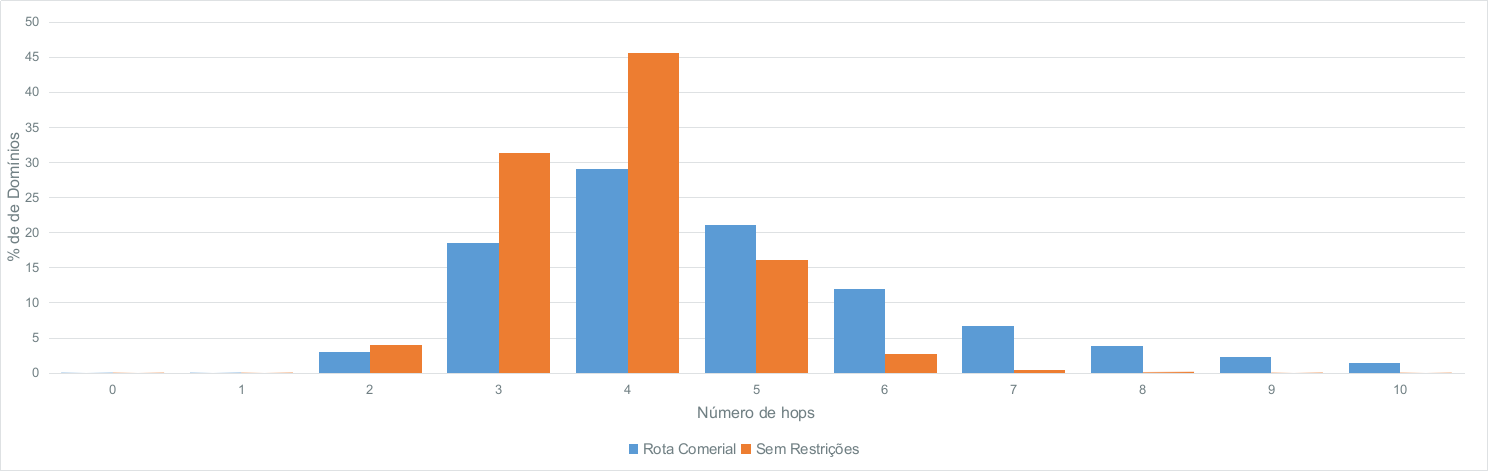
\includegraphics[width=\textwidth]{grafico.png}
	\caption{Percentagem de domínios que chega ao destino com \textit{x} hops com e sem restrições comerciais}
\end{figure}

O algoritmo utilizado para calcular os caminhos mais curtos sem nenhuma restrição foi uma BFS sem qualquer modificação que avalia os domínios a partir da origem. A sua complexidade é também $\mathcal{O}(m+n)$ uma vez que se percorrem todos os domínios e suas ligações uma e uma só vez. Tanto este algoritmo como o \texttt{CommercialRouteHops} foram executados $n$ vezes, uma vez que se calculou a distância de todos os domínios para todos os outros.

Verifica-se que as comunicações na Internet percorrem substancialmente mais domínios para atingir o destino do que aqueles que são fisicamente possíveis. Isto porque a distribuição do gráfico é mais concentrada para os caminhos mais curtos sem restrições.

No gráfico apenas está representado o numero de hops até um máximo de 10. No entanto, são necessários 11 hops para chegar a todos os domínios sem restrições e 35 tendo em conta as restrições comerciais. Optou-se por não representar a totalidade dos 35 hops por não haver relevância percentual, ou seja apenas 2,7\% dos dominios necessita entre 11 a 35 hops para chegar ao destino, tenho em conta as restrições comerciais.


\end{document}
